\section{VGA}
    \tab Jak widać na zdjęciu \ref{fig:mimas}, płytka \underline{nie} jest wyposażona we wbudowane złącze VGA,
    wymagane więc dołożenia zewnętrznego złącza, oraz rezystorów szeregowych, 
    pozwalających na spełnienie standardu napięć VGA. Poniżej przedstawiono schemat połączeń jakie należy wykonać.

    \begin{figure}[!ht]
        \centering
        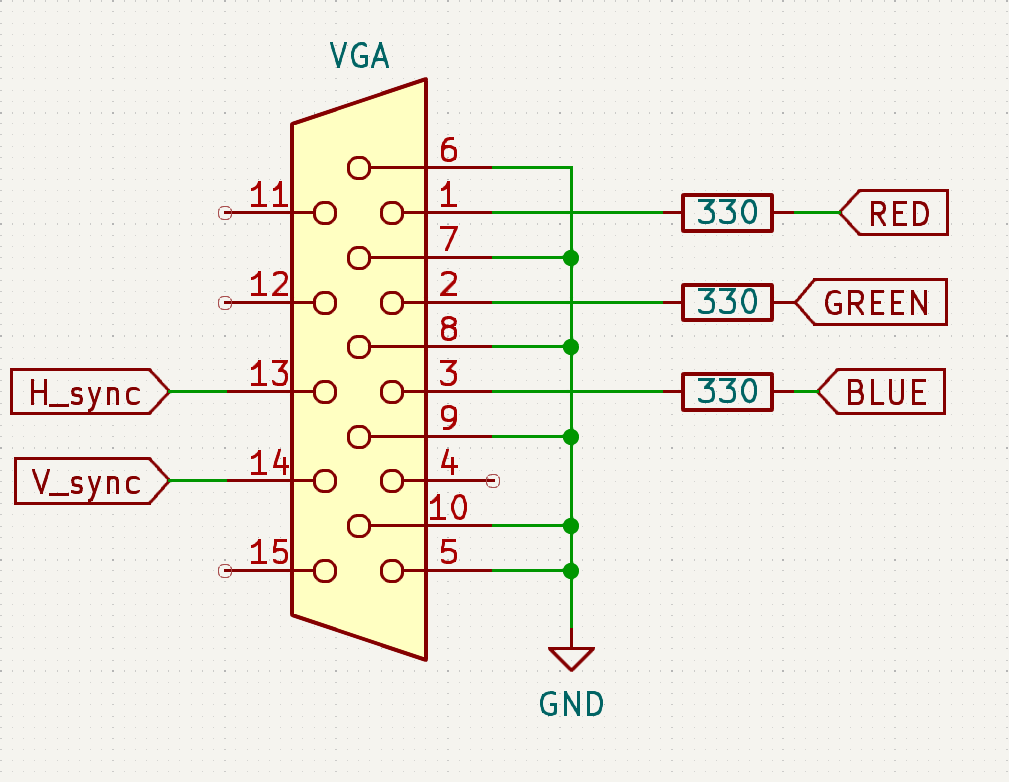
\includegraphics[width = 0.7\textwidth]{VGA.png}
        \renewcommand{\figurename}{Schemat}
        \caption{Złącze VGA}
    \end{figure}

    Zgodnie ze standardem, zakres napięć ograniczony jest od dołu: $0V$ (pełna czerń) do maksymalnie: $0.7V$ (pełen kolor).
    Dodatkowo, impedancja wejściowa oscyluje w okolicy $75\Omega$. 
    A więc dołączenie sygnału o napięciu $3.3V$ przez rezystor o wartości $\ge 280\Omega$ pozwala dostosować progi napięciowe do standardu, zgodnie ze wzorem (\ref{equ:voltage_devider}):
    
    \begin{equation}
        V_o = V_i \cdot \frac{75\Omega}{75\Omega + R_{\text{color}}}
        \label{equ:voltage_devider}
    \end{equation}
    % W projekcie zostały wykorzystane rezystory z szeregu E24, o wartości większej od przyjętej minimalnej - $330\Omega$

    Poniżej przedstawiono schemat blokowy modułu odpowiadającego za synchronizację sygnałów VGA:
    \begin{figure}[!ht]
        \centering
        \begin{circuitikz}
            \draw
                (0, 0) node [draw, align=center, minimum width = 4cm] (H_cnt){Licznik horyzontalny\\$mod\ 800$}
                (6, 0) node [draw, align=center, minimum width = 4cm] (V_cnt){Licznik wertykalny  \\$mod\ 525$}
                (H_cnt.west) to[short, i<=\ , -o] (-3, 0) node[left]{25MHz}
                (H_cnt.east) to[short, i>=Reset] (V_cnt.west)

                (7, -1.75) node[and port, number inputs=3, anchor = out](color_en){}

                (-3, -2) coordinate(color) node[left]{Color}
                (color) to[short, o-, tmultiwire] ++ (2, 0) -- (color_en.in 3)
                (color_en.out) to[short, -o, tmultiwire] ++ (1.5, 0) node[right]{RGB}
                (H_cnt.south) ++ ( 0, 0) -- (0, -1.75) to[short, i=Draw Enable] (color_en.in 2)
                (V_cnt.south) ++ (-1, 0) to[short, i=Draw Enable] ++ (0,-0.95) -- (color_en.in 1)

                (H_cnt.south) ++ ( 1, 0) |- (8.5,-1.25) to[short, -o] ++ (0, 0) node[right]{$H_{sync}$}
                (V_cnt.south) ++ ( 1, 0) |- (8.5,-0.75)    to[short, -o] ++ (0, 0) node[right]{$V_{sync}$}

            ;
        \end{circuitikz}
        \renewcommand{\figurename}{Schemat}
        \caption{Schemat blokowy VGA}
        \label{schematic:VGA}
    \end{figure}



